\documentclass[10pt,twocolumn]{icfd2026paper}
\usepackage[dvipdfmx]{graphicx}
\usepackage{ascmac}
\usepackage{amsmath,amssymb}
\usepackage{indentfirst}
\usepackage{newtxtext,newtxmath} %change font 2025/05/09
\usepackage[backend=biber, style=nature]{biblatex}
\addbibresource{biblio.bib}

\newcommand{\bm}[1]{\mbox{\boldmath{${#1}$}}}
\newcommand{\pd}[2]{{\frac{\partial {#1}}{\partial {#2}}}}
\newcommand{\pdd}[2]{{\frac{\partial^2 {#1}}{\partial {#2}^2}}}
\newcommand{\od}[2]{{\frac{{\rm{d}} {#1}}{{\rm{d}} {#2}}}}
\newcommand{\odd}[2]{{\frac{{\rm{d}}^2 {#1}}{{\rm{d}} {#2}^2}}}


%%% Title %%% 
% Please capitalize the first letter of each major word in the title.
\title{Importance of N2Hx Reaction Pathways in Modelling of NH3/H2/Air Flame Chemistry}

%%% Names of author(): Firstame Familyame %%%
% Please underline the presenter using \underline
\author{\underline{Aahil Ashraf Urothiyil}${}^1$,
	Abe Shunnosuke${}^1$, Matsuda Dai${}^1$, Kitagawa Toshiaki${}^1$, Ekenechukwu Chijioke Okafor${}^1$
	%%% Email address of the corresponding author %%%
	%\footnote for corr. author & e-mail should be placed after the last author
	%
	\footnote{\normalsize Corresponding author: Aahil Urothiyil}
	\footnote{\normalsize {\textit{E-mail address}}:  urothiyil.aahil.412@s.kyushu-u.ac.jp}
	\\
	%%% Affiliation(s) and address %%%
	${}^1$Department of Mechanical Engineering, Kyushu University \\
	7-4-4, Motooka, Nishi-ku, Fukuoka, 819--0395, Japan \\
	% 2-1-1, Katahira, Aoba-ku, Sendai, Miyagi 980--8577, Japan \\
	${}^1$Student \\ % Affiliation
	Street, City, State, Zip-code, Country
}
%%%
\abstract{

	To investigate the importance of N2Hx reaction pathways in modelling NH3/H2/Air flames, the LBV of the mixture was
	modelled using an existing reaction mechanism. This mechanism reproduced LBV of NH3/Air and NH3/CH4/Air flames
	accurately as the mechanism was optimized and validated for these fuel blends however, LBV of NH3/H2/Air were
	under-predicted. Comparing reaction pathways and LBV sensitivities of other mechanisms that were optimized for
	NH3/H2/Air, the importance of N2Hx reaction pathways was established. A present mechanism was developed and then
	validated with data from literature.
	
}
\pagestyle{empty}

\begin{document}

\maketitle
\thispagestyle{empty}

\section{Introduction}

Ammonia has gained interest as a carbon free fuel for combustion systems and the blending of ammonia with other
faster burning fuel, such as methane and hydrogen, is a means considered for improving the combustion characteristics of
ammonia mixtures. To further study the phenomena observed with the combustion of ammonia and its blends under variying
conditions, numerical simulations with chemical kinetics mechanisms in neccessary. These choice of mechanisms determine
the accuracy of the numerically simulated flames. Reaction mechanisms that are able to accurately predict parameters of
the flame, such as laminar burning velocity (LBV), under varying conditions, like rich/lean equivalence ratio and
varying fuel compositions, is desired.

Many chemical kinetic mechanisms that model NH3/Air flames or specific blends of ammonia exist. Most of these
mechanisms were developed, optimized and validated for targeted mixtures, specific set of flame characteristics and
select experimental conditions. Okafor Reduced mechanism, for instance, ...

The aim of this study is to develop a reaction mechanism to accurately model flames for ammonia and ammonia blends
--- namely NH3/H2/Air and CH4/NH3/Air flames. This mechanism prioritizes LBV, a critical flame characteristic that
dictates fuel compatability for a wide range of practical applications. Most existing reaction mechanisms from
literature are only able to reproduce some fuels' LBV accurately under select pressure, initial temperature and
equivalence ratios. Okafor Reduced mechanism, for example, is designed to predict CH4/NH3/Air's LBV. This mechanism also
exhibits high reproducibility for LBVs of NH3/Air flames and H2/Air flames however underpredicts LBV of NH3/H2/Air
flames. In this study, the reason for the underprediction was studied and a mechanism was developed around the findings.

\section{Developing Reaction Mechanism}

The new reaction mechanism developed in this paper was based on the Okafor Reduced mechanism. Okafor reduced
mechanism was selected because this mechanism has been optimized and validated for LBV prediction of NH3/Air and
NH3/CH4/Air flames. This is true for varying equivalence ratios, pressures and, in the case of NH3/CH4/Air flames,
varying methane concentrations. This mechanism also models the LBV of H2/Air flames satisfactorily for most of these
conditions. This mechanism performs poorly when the it is used to predict LBV of NH3/H2/Air flames at hydrogen
concentrations greater than 0.3. The mechanism's failure to predict the LBV for this specific blend, despite accurately
reproducing the individual components of NH3/H2/Air flames, motivated the current investigation. Correcting this
discrepancy brings this mechanism to fulfil the aim of this study.

[Figure: lbv NH3, H2, NH3/H2]
\begin{figure}[ht]
\begin{center}
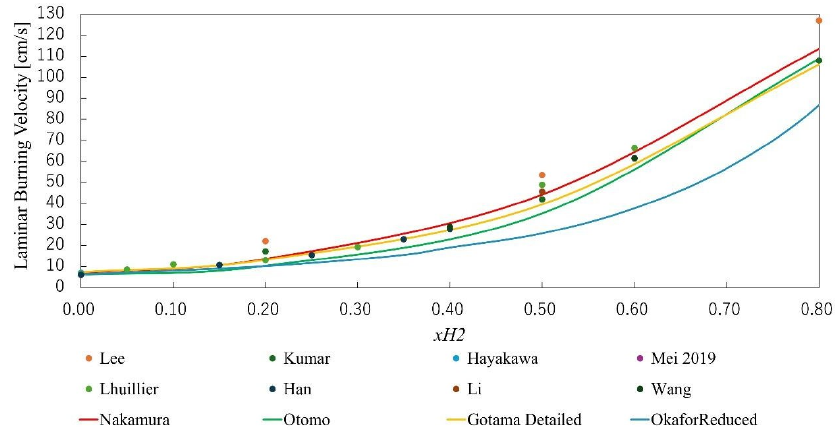
\includegraphics[width=8.0cm,keepaspectratio]{figures/lbv_nh3-h2.png}
\end{center}
\caption{
	Experimental and numerical laminar burning velocity of NH3/H2/Air flames under stoichiometric condition at various
	hydrogen concentrations}
\label{fig-lbv_nh3-h2}
\vspace{2mm}
\end{figure}

Nakamura Mech \cite{nakamuraKinetic2017} is one of the mechanisms studied to develop the Present Mech and the
mechanism on NH3/Air flames. This mechanism was selected because Nakamura et al. identifies the important role N2Hx
species play in the ignition of NH3/Air flames, especially at lower temperatures \cite{nakamuraCombustion2017}. Hence,
the mechanism has a detailed description of how N2Hx species interact with intermediate species and radicals to control
the reactivity of ammonia. Moreover, Nakamura Mech's predictions for NO and N2O molar fractions, downstream of the
reaction zone, laminar burning velocity and ignition delay time agree satisfactorily with data from literature.

Another mechanism that was studied to develop the Present Mech was Gotama Mech \cite{gotamaMeasurement2022}.
This mechanism was developed to model NH3/H2/Air flames for laminar burning velocity. Gotama et al. re-emphasizes the
importance of N2Hx reaction pathways in the combustion of flames containing ammonia. The author outlines an H2 recovery
mechanism in which NH3 and H2 kinetics are coupled to regulate H radical and H2 concentrations \cite{otomoChemical2018}.
Using this mechanism, Gotama Mech is able to accurately model NH3/H2/Air flames at varying hydrogen concentrations.
Implementing the H2 recovery mechanism could improve Present Mech's NHx and N2Hx kinetics for flames with different
hydrogen concentrations.

\subsection{Methodology}

Numerical simulations for this study is conducted using ANSYS Chemkin-PRO 2019 R3 and ANSYS Chemkin 2025 R2. The
"Premixed Laminar Flame Speed Calculation" model was used and the initial conditions kept constant for all the
simulations were the pressure at 1.0 atm, temperature at 298.0 K, and equivalence ratio at 1.0. To study the effects of
hydrogen addition to the blend, the simulations were run with fuel composed of xH2=0.5 and xNH3=0.5. xH2=0.5 was
selected to compare these mechanisms as Nakamura Mech and Gotama Mech estimate LBV with reasonable accuracy at these
conditions and Okafor Reduced Mech deviates significantly from the experimantal LBV at this ratio. The computational
domains was set to 10 cm and the solver properties GRAD and CURV were set to 0.01. Multicomponent transport and thermal
diffusion --- Soret effect --- was enabled.

After simulating the flames with the settings metioned, reaction pathways were created using integrated rate of
production (IROP) of each elementary reaction in the mechanisms. Rate of production (ROP) is evaluated at each space
step in the computational domain and proves to be a difficult parameter to use to compare elementary reactions of
different mechanisms because different reactions' ROPs peak along different points in the domain. To address this
limitation, ROP of each elementary reaction is integrated along its domain (\ref{eqn:irop}) resulting in one number to
represent an elementary reaction's ROP across the domain. 

\begin{eqnarray}
	IROP=\int_0^L\dot\omega_{R,i}\text dx
	\label{eqn:irop}
\end{eqnarray}

For Okafor Reduced Mech, IROPs are then normalized with respect to the IROP of the OH$\rightarrow$H2O pathway, the
reaction pathway with the highest. The normalized IROPs are used to draw the reaction pathways and the normalized IROP
value for each pathway determine the thickness of the line. Gotama and Nakamura Mechs will use "Relative Size", the IROP
of the pathway relative to Okafor Reduced Mech, to determine the line thicknesses in their reaction mechanisms.

Then the normalized sensity of burning velocity, and mole fractions of species of interest, with respect to the
rate constants of the elementary reactions were evaluated for Okafor Reduced Mech and the Present Mech. The species of
interest were H, OH, NH, NH2, N2H2, NNH and N2H3 as these intermediate species were identified to be significant in
NH3/H2 flame chemistry. The sensitvity coefficients represent how the A-factors of each elementary reaction impacts the
parameters ---  LBV or the species mentioned. Comparing the sensitivity analysis plots give insights into which
elementary reactions are significant with respect to each parameter and how they affect the parameters in the updated
Present Mech.

% Instead of "sensitivity analysis" it is "normalized sensitivity of the burning velocity with respect to the rate
% constants of the elementary reactions"
% Explain IROP in its entirety and the reason why IROP was used in this instance
% Explain sensitivity analysis in its entirety and the reason why it was used in this instance

\subsection{Findings from Comparing Mechanisms}

[Figures reaction pathways]
\begin{figure}[ht]
\begin{center}
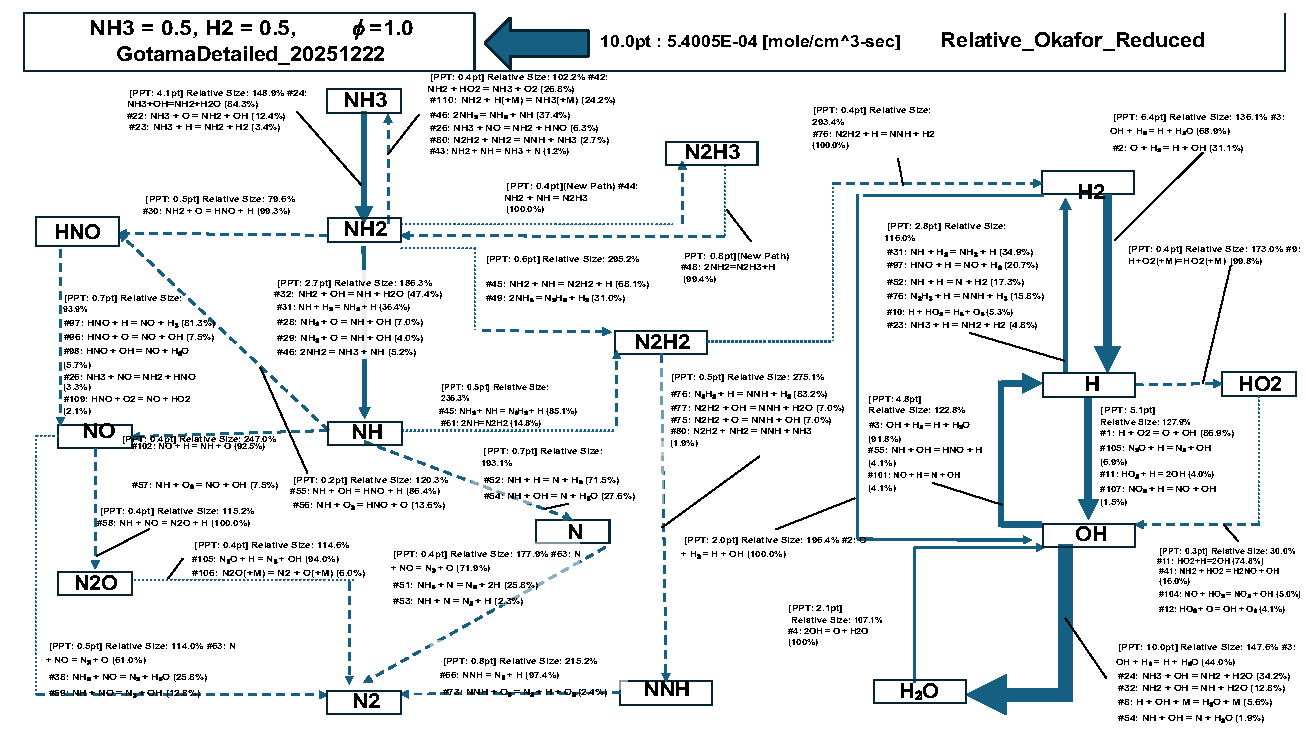
\includegraphics[width=8.0cm,keepaspectratio]{figures/gotama_reaction-pathways.png}
\end{center}
\caption{Reaction pathway of NH3/H2/Air flame at xH2=0.5 and equivalence ratio of 1.0 using Gotama Detailed Mechanism}
\label{fig-gotama_reac-path}
\vspace{2mm}
\end{figure}

With Okafor Reduced Mech and Gotama Mech, NH3/H2/Air flames were numerical simulated under conditions and setup
outlined in the Methodology. IROPs for both mechanisms were calculated and was used to construct Fig
\ref{fig-gotama_reac-path}, a reaction pathway comparing each Gotama Mech pathway to the corresponding Okafor reduced
Mech pathway. The most notable pathway in Fig \ref{fig-gotama_reac-path} is NH2$\leftrightarrow$N2H3 which is only
significant in Gotama Mech. The forward reaction, the formation of N2H3, is given by NH2+NH=N2H3 (R1) and the reverse, the
consumption of N2H3, is given by 2NH3=N2H3+H (R2). These reactions affect the concentrations of NH and NH2, which are key
intermediates in the ammonia oxidation pathway. The inclusion of these reactions suggests that the LBV would be promoted
and could be why Okafor Reduced Mech, lacking these pathways, under-predicts LBV at intermediate xH2.

Other pathways that have a significantly higher IROP in Gotama Mech's reaction pathway are the
NH3$\rightarrow$NH2$\rightarrow$N2H2$\rightarrow$NNH$\rightarrow$N2 as can be noticed in Fig.
\ref{fig-gotama_reac-path}. From this pathway, the NNH->N2 pathway, which has an IROP 2.2 times greater in Gotama Mech's
pathway relative to Okafor Reduced Mech, is facilitated primarily by the reaction NNH=N2+H (97.4\%) (R3). This finding
suggests that more H radicals are produced by Gotama Mech through this pathway, relative to Okafor Reduced Mech, and
correlates with the higher LBV prediction with Gotama Mech. 

The prior observation can also be found in the
NH3$\rightarrow$NH2$\rightarrow$NH$\rightarrow$N2H2$\rightarrow$NNH$\rightarrow$N2 pathway. IROPs for these pathways are
greater in Gotama Mech's reaction pathway than Okafor Reduced Mech's pathway. Furthermore, another H radical generating
reaction from this pathway, specifically the NH2$\rightarrow$NH pathway, also suggests strong correlation with
increasing LBV. This reaction is NH2+NH=N2H2+H (R4), which also includes NH and NH2, important intermediate species that
affect LBV.

(*4) The three observations from Fig. \ref{fig-gotama_reac-path} depict the importance N2Hx species and their reaction
pathways have on LBV prediction accuracy. Okafor Reduced Mech's LBV under-prediction for NH3/H2/Air flames at
intermediate hydrogen concentrations has a correlation with N2Hx reaction pathways omitted or poorly modelled. This led
us to believe that formation and consumption reactions of NH2 and NH were not accurately represented, resulting in poor
flame modelling under these conditions. N2Hx reaction pathways also displayed involvement in H radical generation which
correlated with LBV prediction.

(*4) The comparison between Nakamura Mech and Okafor Reduced Mech reaction pathways was also
conducted. Significant differences in IROP of certain pathways with reactions containing NO and this could be linked to
the increased concentration of H radicals due to hydrogen co-combustion. More H radicals lead to increased production of
O and OH radicals, radicals that activate reaction pathways containing NO. NH$\rightarrow$N pathway has a higher IROP in
Nakamura Mech's reaction pathway due to the influx of H radicals. The excess N being produced as a result of this,
paired with NO, reaction N+NO=N2+O facilitates the IROP increase in N$\rightarrow$N2 reaction pathway in Nakamura
Mech. However, NO-related pathways from Nakamura were not incorporated into Present Mech as insights from Okafor Reduced
Mech's LBV of oxygen-enriched combustion \cite{abe}. Under such conditions, O and OH radicals are in abundance too
however, Okafor Reduced Mech predicted LBV accurately leading us to determine updating the NO-related pathways were of
low priority.

\subsection{Changes in the New Mechanism}

Since N2Hx reaction pathways are demonstrated to be consequential to LBV modelling by the comparison of Gotama
Mech's and Okafor Reduced Mech's reaction pathways for an NH3/H2/Air flame, Gotama Mech was used to inform the updates
made to Present Mech. Present Mech focuses on better describing N2Hx-related reaction pathways in the chemical kinetics
mechanism. This was achieved by focusing on two aspects of the reaction pathway: N2Hx reactions in the
NH2$\rightarrow$NH pathway and N2Hx formation/consumption to convert NHx radicals to NNH. Therefore reactions pertaining
to species NH2, NNH, N2H2 and N2H4 from Gotama Mech were incorporated into Okafor Reduced Mech to form Present Mech.

[Figure new Mech lbv]
\begin{figure}[ht]
\begin{center}
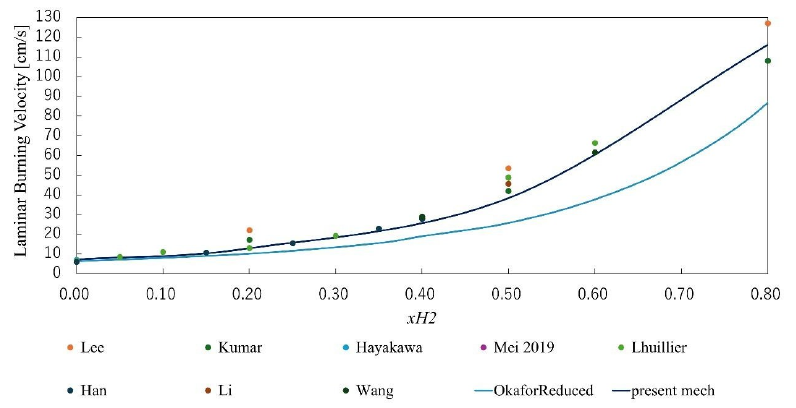
\includegraphics[width=8.0cm,keepaspectratio]{figures/lbv_present_nh3-h2.png}
\end{center}
\caption{Experimental and numerically calculated laminar (Present Mech and Okafor Reduced Mech) burning velocity of NH3/H2/Air flames
under stoichiometric condition at various hydrogen concentrations}
\label{fig-lbv_present}
\vspace{2mm}
\end{figure}

Figure \ref{fig-lbv_present} compares the LBV predictions of Present Mech to Okafor Reduced Mech and experimental data
from literature under the same conditions the reaction pathway analysis was conducted in. It is evident that the changes
made to the Okafor Reduced Mech have been effective to bring calculated LBV for fuel compositions with intermediate
and high hydrogen concentrations are closer to real flames' LBV. Further validation will be conducted in this paper to
ensure Present Mech fulfils the full scope this study's aim.

\section{Analysis of NH3/H2/Air Flame Characteristics}

\subsection{Sensitivity Analysis With Respect to Laminar Burning Velocity}

[Figure lbv sens analysis]
\begin{figure}[ht]
\begin{center}
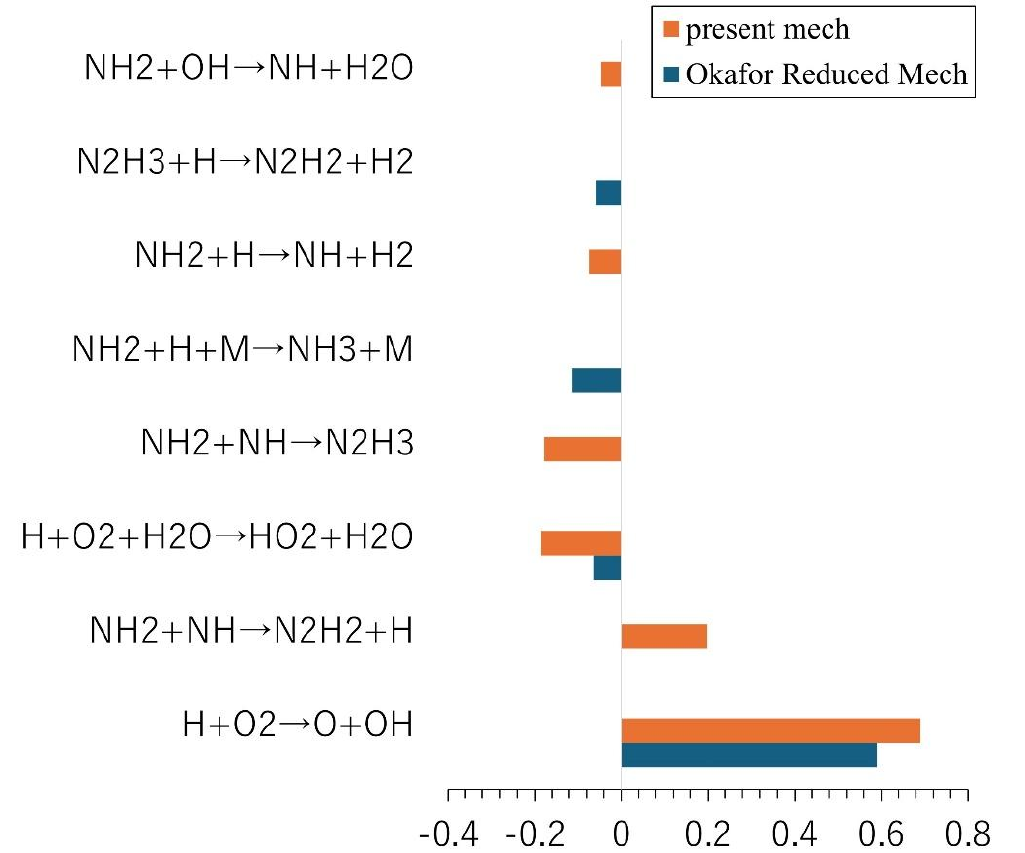
\includegraphics[width=7.0cm,keepaspectratio]{figures/lbv_sens.png}
\end{center}
\caption{sensitivity coefficients for laminar burning velocity of NH3/H2/Air flames at xH2=0.5 and equivalence ratio of
1.0 under atmospheric conditions.}
\label{fig-lbv_sens}
\vspace{2mm}
\end{figure}

From Fig. \ref{fig-lbv_sens}, reaction (R4), NH2+NH=N2H2+H, plays a significant role in promoting LBV in Gotama
Mech whereas is not significant in Okafor Reduced Mech. Such a pattern can also be noticed in one of the reaction
primarily responsible for inhibiting LBV in Gotama Mech, NH2+NH=N2H3 (R1). The figure also shows other NHx and N2Hx
related reactions being more significant with respect to LBV in Present Mech, suggesting the dominant role these species
play in controlling the LBV of an NH3/H2/Air flame, at intermediate hydrogen concentration, has been modelled.

\subsection{Sensitivity Analysis With Respect to Major Chemical Species}

NHx species, like NH and NH2 radicals, mole fractions sensitivity to elementary reactions' A-factors are plotted in
[fig nhx sens]. Both, Okafor Reduced Mech and Present Mech, agree that the reaction NH3+OH$\rightarrow$NH2+H2O (R5) and
the reaction NH2+H$\rightarrow$NH+H2 (R6) are the major reaction involved in NH3 and NH2 consumption respectively.
However, Present Mech also identifies the reaction NH2+OH$\rightarrow$NH+H2O (R7) significantly contributes to NH2
consumption as depicted in [fig nhx sens]. Reaction (R7) displays negative sensitivity to NH2 mole fraction with both
mechanisms while exhibiting significant, positive sensitivity with Present Mech to NH mole fraction. Thus, Present Mech
promotes NH consumption via reaction (R7). Reaction NH+H$\rightarrow$N+H2 (R8), on the other hand, exhibits significant
negative sensitivity to NH mole fraction, suggesting that (R8) is the primary decomposition pathway for NH.

On the other hand, N2Hx species, as shown in [fig n2hx sens], depend on NHx radicals to recombine and form NNH,
N2H2 or N2H3. NNH and N2H2 mole fraction exhibits dependance on reaction (R4), NH2+NH=N2H2+H, wheras N2H3 mole fraction
is negatively impacted by the same reaction. The negative sensitivity coefficient for N2H3 mole fraction is because N2H3
relies on the same reactants, NH and NH2, in reaction (R1), NH2+NH=N2H3. Since H radical generation is significant via
(R1) in NH3/H2/Air flames with intermediate xH2, both reactions are competing for the NH and NH2 radicals. Reaction (R4)
activates the reaction zone whereas reaction (R4) suppresses the reaction zone therefore, both (R1), (R4) and other
reactions governing N2H3 formation were added to Present Mech ensure the reaction zone in balanced in terms of
reactivity. This should in turn improve the LBV prediction accuracy while using Present Mech.

\section{Validation}

\section{Concluding Remarks}



\printbibliography
\end{document}
